\chapter{Limitations, negative evidence와 falsifiers}
\label{STC-S16}

이 Study의 결론은 2026-08-05 공개 evidence에 대한 조건부 synthesis다. Product 내부 trace, 비공개
deployment incident, 실제 device workload가 없으며, 논문 간 model·task·budget이 달라 meta-analysis를
수행하지 않았다. Original figure의 좌표와 scenario는 측정 결과가 아니라 reasoning aid다.

\section{문헌 자체의 한계}

명시적 parametric sleep 연구는 direct mechanism evidence지만 model scale, task diversity, cycle count와
production governance가 제한된다. Product documentation은 background phase의 존재를 보여도 strongest
alternative 대비 causal advantage를 보여 주지 않는다. Continual-learning precursor는 forgetting을 줄이는
방법을 제공하지만 LLM agent의 deletion, state migration, future reuse economics를 직접 측정하지 않는다.

DANN/SSRN record는 동결 source에서 independent verification에 필요한 method와 result를 충분히 공개하지
않아 load-bearing evidence로 사용하지 않았다.\claim{STC-C047}\autocite{srcstc0039} 제목이나 abstract가
``zero forgetting''을 말해도 full method, data, comparator, statistics, artifact가 없으면 central claim을
지탱할 수 없다. 이 판단은 논문이 틀렸다는 결론이 아니라 증거 접근성에 대한 claim-down이다.

\section{Negative evidence가 가리키는 구조적 위험}

\begin{longtable}{L{0.20\textwidth} L{0.31\textwidth} L{0.39\textwidth}}
\caption{실패 mode와 필요한 control}\label{tab:negative-evidence}\\
\toprule
Risk & 관찰/이론적 근거 & 필요한 control \\
\midrule
\endfirsthead
\toprule
Risk & 관찰/이론적 근거 & 필요한 control \\
\midrule
\endhead
behavioral unreachability & sequential fact가 weights에 남아도 normal query에서 접근 불가 & direct, prompted, compositional reachability를 분리 \\
catastrophic interference & new update가 old task와 plasticity를 손상 & old/new/safety slice, replay/regularization/isolation ablation \\
recursive-data collapse & synthetic-only generations가 rare tail을 잃을 수 있음 & canonical anchor, recursive depth, common/tail distortion \\
false merge/compaction & summary가 exact, temporal, negative detail을 지움 & source spans, faithfulness, exact/temporal query, rebuild \\
memory poisoning & persistent record가 후속 behavior를 조종 & provenance, quarantine, poison canary, least privilege \\
delete illusion & tombstone 뒤 summary, index, cache, adapter에 영향 잔존 & lineage fan-out, deny root, physical removal, residual probe \\
state fan-out & user/cohort artifact와 catalog가 base saving을 상쇄 & total state, hot residency, route/load latency \\
queue/SLA failure & 평균 utilization 전에도 affinity·validation이 P99 age를 악화 & multi-resource queue, deadline, wake preemption \\
version churn & base/tokenizer/embedding 변경이 artifact를 무효화 & compatibility digest, rebase/rebuild cost \\
\bottomrule
\end{longtable}

\begin{figure}[htbp]
  \centering
  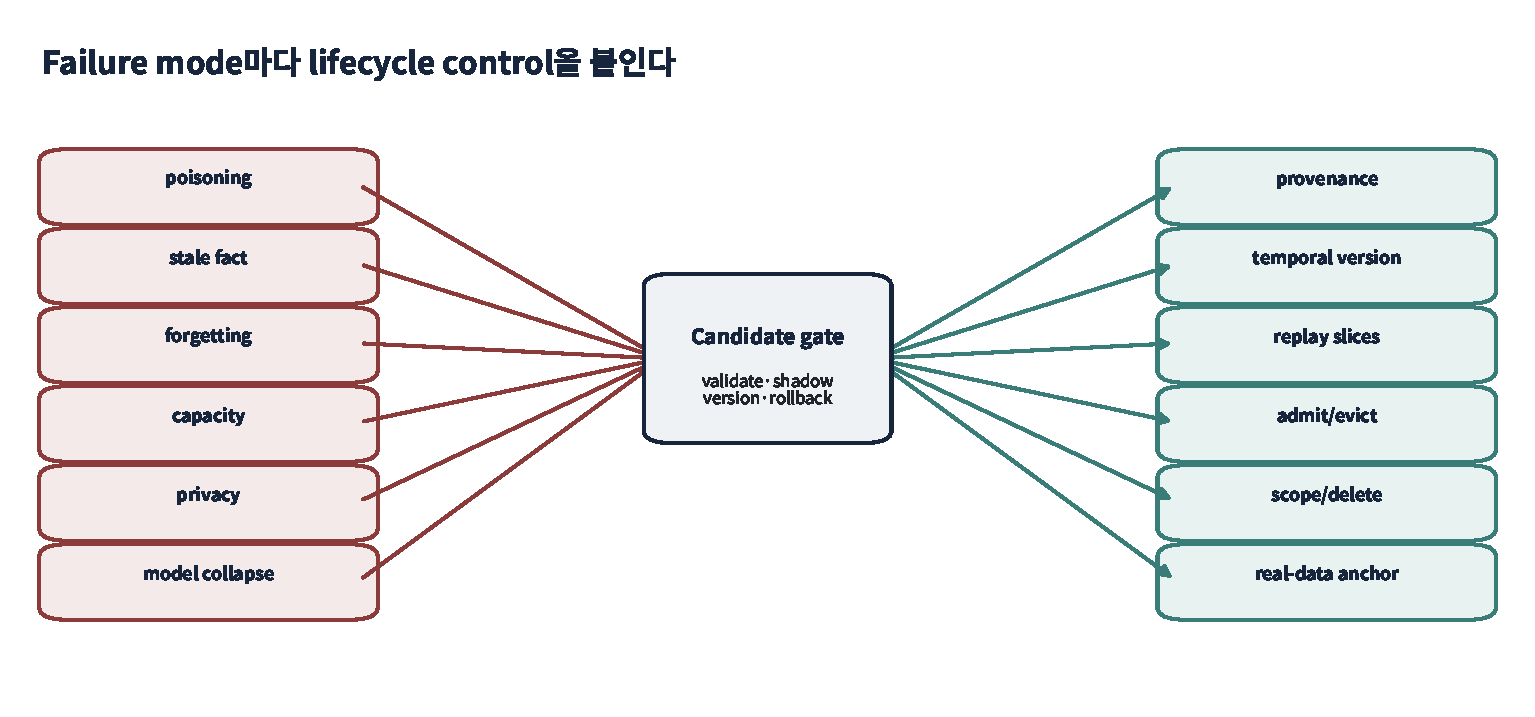
\includegraphics[width=0.98\textwidth]{figures/stc-f013.pdf}
  \caption{Wake capture에서 deletion까지 이어지는 주요 failure mode와 lifecycle control. 한 단계의
  accuracy gate만으로는 poison, stale publish, rollback resurrection, residual delete를 막을 수 없다.}
  \stcfigure{STC-F013}
  \figsource{Original synthesis; SRC-STC-0042, SRC-STC-0053}{Admission, candidate, publish, serve, delete 단계마다 poison·interference·race·residual과 대응 control을 연결한 흐름도.}
  \label{fig:failure-controls}
\end{figure}

\section{결론을 뒤집거나 좁힐 구체적 falsifier}

\textbf{F1---새 phase claim.} 동일 transformation, information cutoff, destination, total resource를
맞췄을 때 deferred와 synchronous 실행의 later-wake quality, wake-SLA, batching 차이가 모두 사라지면
``새 scientific axis''는 scheduling label로 좁혀야 한다.

\textbf{F2---hybrid recommendation.} External-only 또는 direct parametric-only가 stable skill과 volatile
fact 모두에서 utility, cost, deletion, rollback, portability를 지배하면 hybrid default를 폐기한다.

\textbf{F3---valid-reuse hypothesis.} Reuse와 query predictability를 넓게 sweep해도 STC gain과 interaction이
없거나 predictor error가 top-$k$ yield를 없애면 reuse-based promotion 이론을 기각한다.

\textbf{F4---capacity knee.} Repeated stream에서 behavioral retention/plasticity가 physical occupancy와
같이 부드럽게 변하고 앞선 knee가 재현되지 않으면 별도 behavioral knee hypothesis를 기각한다.

\textbf{F5---canonical anchoring.} Synthetic/summary replay와 source-anchored replay의 rare-tail survival이
matched cost에서 차이가 없으면 canonical anchor의 안정성 주장을 낮춘다.

\textbf{F6---dedicated sleep infra.} Shared priority fleet가 모든 realistic trace에서 더 낮은 physical
peak, 이동 bytes, P99 wake latency와 job age를 동시에 보이면 separate sleep cluster 필요성을 기각한다.

\textbf{F7---device relevance.} Background memory job이 commodity CPU/object-store metadata 수준에 머물고
retained bytes, rewrite, movement, tail-SLA가 장치 선택에 영향을 주지 않으면 새로운 memory workload라는
주장을 좁힌다.

\section{Coverage와 saturation의 한계}

Search cluster는 date-bounded snapshot이며 five active frontier와 five measurement gap을 명시적으로
남겼다. 특히 Google, Meta, Microsoft의 research output은 넓지만 public production per-user weight sleep의
부재를 ``그 회사가 하지 않는다''는 negative fact로 바꾸지 않는다. 공개하지 않았을 가능성과 아직
측정하지 않은 possibility가 있기 때문이다.

Figure는 권리 검토된 original redraw만 사용했으며 source paper figure를 직접 복제하지 않았다. 이
선택은 copyright risk를 줄이지만 원 실험 plot의 numeric fidelity를 대신하지 않는다. 독자는 claim
ledger와 primary source로 수치를 확인해야 한다.

\section{본 논문이 주장하지 않는 것}

\begin{itemize}
  \item Biological NREM/REM stage가 AI operator에 one-to-one으로 대응한다는 주장,
  \item 더 많은 sleep FLOPs가 항상 utility를 높인다는 universal monotone law,
  \item weights가 external memory보다 본질적으로 더 장기적이라는 주장,
  \item 공개 product lifecycle가 comparative scientific optimality를 입증한다는 주장,
  \item simulation이 특정 GPU·memory device의 latency, energy, endurance를 측정했다는 주장,
  \item P3-held device hypothesis가 publication 또는 patent review를 통과했다는 주장.
\end{itemize}

\begin{cautionbox}[가장 중요한 한계]
현재 논문은 measurement program과 conditional strategy를 제시한다. STC의 universal dominance나 broad
parametric deployment를 관측한 논문이 아니다. 이 구분을 유지해야 향후 negative result가 연구 실패가
아니라 이론의 경계를 좁히는 결과가 된다.
\end{cautionbox}
